\documentclass[10pt]{article}
\usepackage[utf8]{inputenc}
\usepackage{amsmath,graphicx}
\usepackage{amsthm,amssymb,mathtools}
\usepackage{tikz}

\begin{document}

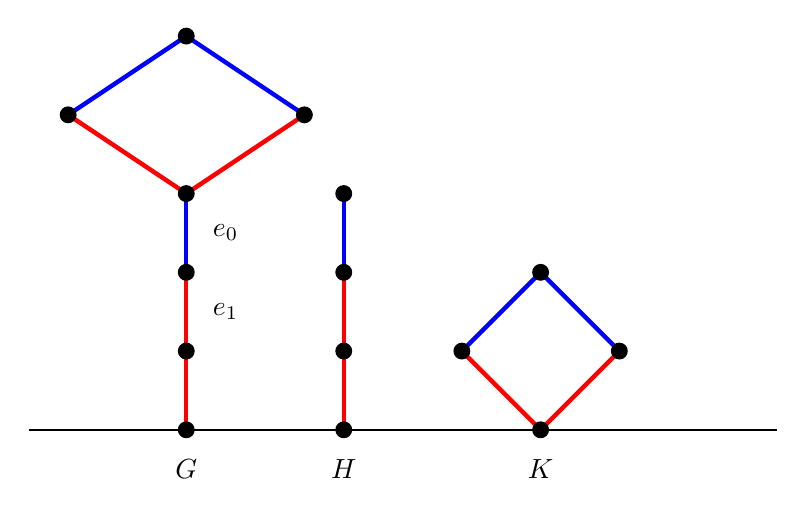
\begin{tikzpicture}

 \draw[thick,black] (8.5,0) -- (18,0);

 	\node[fill=none] at (10.5,-0.5) (nodes) {$G$};
	\draw[ultra thick,red](10.5,0)--(10.5,1);
	\draw[ultra thick,red](10.5,1)--(10.5,2);
 	  \node[fill=none] at (11,1.5) (nodes) {$e_1$};
	\draw[ultra thick,blue](10.5,2)--(10.5,3);
 	  \node[fill=none] at (11,2.5) (nodes) {$e_0$};
	\draw[ultra thick,red](10.5,3)--(9,4);
	\draw[ultra thick,blue](9,4)--(10.5,5);
	\draw[ultra thick,blue](10.5,5)--(12,4);
	\draw[ultra thick,red](12,4)--(10.5,3);
 
	\filldraw[black] (10.5,0) circle [radius=1mm];
   	\filldraw[black] (10.5,1) circle [radius=1mm];
   	\filldraw[black] (10.5,2) circle [radius=1mm];
   	\filldraw[black] (10.5,3) circle [radius=1mm];
   	\filldraw[black] (10.5,5) circle [radius=1mm];
   	\filldraw[black] (9,4) circle [radius=1mm];
   	\filldraw[black] (12,4) circle [radius=1mm]; 


    \node[fill=none] at (12.5,-0.5) (nodes) {$H$};
	\draw[ultra thick,red](12.5,0)--(12.5,1);
	\draw[ultra thick,red](12.5,1)--(12.5,2);
	\draw[ultra thick,blue](12.5,2)--(12.5,3);

    \filldraw[black] (12.5,0) circle [radius=1mm];
   	\filldraw[black] (12.5,1) circle [radius=1mm];
   	\filldraw[black] (12.5,2) circle [radius=1mm];
   	\filldraw[black] (12.5,3) circle [radius=1mm];

    \node[fill=none] at (15,-0.5) (nodes) {$K$};
	\draw[ultra thick,red](15,0)--(14,1);
	\draw[ultra thick,blue](14,1)--(15,2);
	\draw[ultra thick,blue](15,2)--(16,1);
	\draw[ultra thick,red](16,1)--(15,0);

    \filldraw[black] (15,0) circle [radius=1mm];
   	\filldraw[black] (15,2) circle [radius=1mm];
   	\filldraw[black] (14,1) circle [radius=1mm];
   	\filldraw[black] (16,1) circle [radius=1mm]; 
    \end{tikzpicture}

\end{document}